\documentclass[border=4pt]{standalone}
\usepackage{tikz}
\usetikzlibrary{shapes.geometric,arrows.meta,positioning,calc}

\definecolor{faithful}{HTML}{2166ac}
\definecolor{traitor}{HTML}{b2182b}
\definecolor{accent}{HTML}{1b7837}
\definecolor{panelbg}{HTML}{fafafa}

\begin{document}
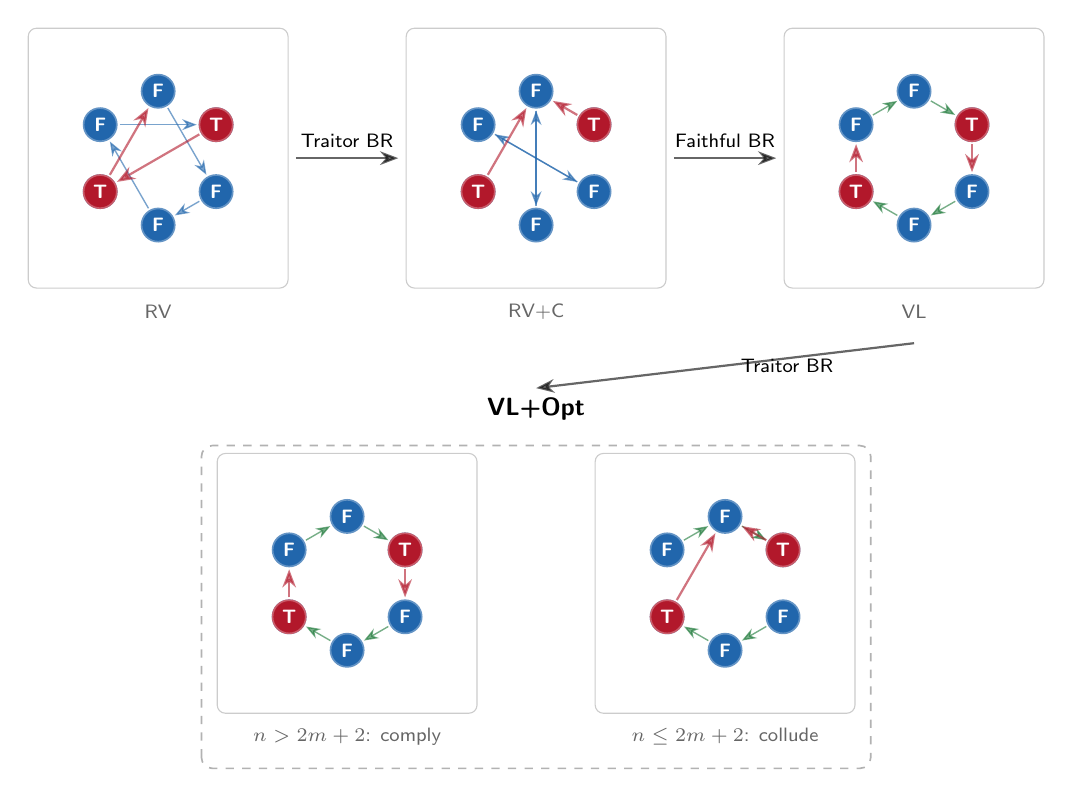
\begin{tikzpicture}[
    >=Stealth,
    font=\sffamily,
    player/.style={circle, minimum size=12pt, inner sep=0pt, line width=0.6pt,
                   font=\sffamily\scriptsize\bfseries, text=white},
    fnode/.style={player, fill=faithful, draw=faithful!70},
    tnode/.style={player, fill=traitor, draw=traitor!70},
    votearrow/.style={->, line width=0.5pt, opacity=0.6,
                      shorten >=7pt, shorten <=7pt},
    caption/.style={font=\sffamily\scriptsize, text=black!60, align=center},
    panelbg/.style={draw=black!20, fill=white, rounded corners=3pt},
]

\def\pw{2.8}    % panel width
\def\ph{5.4}    % vertical spacing between rows (room for down-arrow + label)
\def\R{0.85}    % circle radius for players
\def\xgap{2.0}  % horizontal gap between panels (room for arrows + labels)

% First row panels: 3 panels left-aligned
\coordinate (P1) at (0, \ph);
\coordinate (P2) at (\pw+\xgap, \ph);
\coordinate (P3) at (2*\pw+2*\xgap, \ph);

% Total top-row width: 3*\pw + 2*\xgap. Bottom row spans 2*\pw + \xgap.
% Centre offset = (3*\pw + 2*\xgap - (2*\pw + \xgap)) / 2 = (\pw + \xgap)/2.
% Second row panels: centred under the top row
\coordinate (P4) at ({(\pw+\xgap)/2}, 0);
\coordinate (P5) at ({(\pw+\xgap)/2 + \pw + \xgap}, 0);

% Helper: draw 6 players in a circle
\newcommand{\drawplayerssmall}[3]{
    % #1 = center, #2 = prefix, #3 = comma-separated traitor positions
    \foreach \i in {1,...,6} {
        \pgfmathsetmacro{\angle}{90 - (\i-1)*60}
        \coordinate (#2-\i) at ($(#1) + (\angle:\R)$);
    }
    \foreach \i in {1,...,6} {
        \node[fnode] at (#2-\i) {F};
    }
    \foreach \t in {#3} {
        \node[tnode] at (#2-\t) {T};
    }
}

% ══════════════════════════════════════════════════════════════
% TOP ROW: Three strategies
% ══════════════════════════════════════════════════════════════

% ── Panel A: Random Voting (RV) ──
\begin{scope}[shift=(P1)]
    \draw[panelbg] (-0.25, -0.25) rectangle (\pw+0.25, \pw+0.25);

    \pgfmathsetmacro{\cx}{\pw/2}
    \pgfmathsetmacro{\cy}{\pw/2}
    \coordinate (CA) at (\cx, \cy);
    \drawplayerssmall{CA}{a}{2,5}

    % Random votes: every player votes for a different other player.
    % No bidirectional pairs (otherwise opposite arrows overlap as one line).
    \draw[votearrow, draw=faithful] (a-1) -- (a-3);
    \draw[votearrow, draw=faithful] (a-3) -- (a-4);
    \draw[votearrow, draw=faithful] (a-4) -- (a-6);
    \draw[votearrow, draw=faithful] (a-6) -- (a-2);
    % Traitors vote randomly too: different targets (not colluding)
    \draw[votearrow, draw=traitor, line width=0.8pt] (a-2) -- (a-5);
    \draw[votearrow, draw=traitor, line width=0.8pt] (a-5) -- (a-1);

    \node[caption] at (\pw/2, -0.55) {RV};
\end{scope}

% ── Panel B: Random Voting with Collusion (RV+C) ──
\begin{scope}[shift=(P2)]
    \draw[panelbg] (-0.25, -0.25) rectangle (\pw+0.25, \pw+0.25);

    \pgfmathsetmacro{\cx}{\pw/2}
    \pgfmathsetmacro{\cy}{\pw/2}
    \coordinate (CB) at (\cx, \cy);
    \drawplayerssmall{CB}{b}{2,5}

    % Same random faithful votes
    \draw[votearrow, draw=faithful] (b-1) -- (b-4);
    \draw[votearrow, draw=faithful] (b-3) -- (b-6);
    \draw[votearrow, draw=faithful] (b-4) -- (b-1);
    \draw[votearrow, draw=faithful] (b-6) -- (b-3);
    % Both traitors converge on player 1
    \draw[votearrow, draw=traitor, line width=0.8pt] (b-2) -- (b-1);
    \draw[votearrow, draw=traitor, line width=0.8pt] (b-5) -- (b-1);

    \node[caption] at (\pw/2, -0.55) {RV+C};
\end{scope}

% ── Panel C: Vote-Left (VL) ──
\begin{scope}[shift=(P3)]
    \draw[panelbg] (-0.25, -0.25) rectangle (\pw+0.25, \pw+0.25);

    \pgfmathsetmacro{\cx}{\pw/2}
    \pgfmathsetmacro{\cy}{\pw/2}
    \coordinate (CC) at (\cx, \cy);
    \drawplayerssmall{CC}{c}{2,5}

    % Each votes for next clockwise
    \foreach \i [evaluate=\i as \j using {int(mod(\i, 6) + 1)}] in {1,...,6} {
        \pgfmathsetmacro{\isTraitor}{\i == 2 || \i == 5 ? 1 : 0}
        \ifnum\isTraitor=1
            \draw[votearrow, draw=traitor, line width=0.8pt] (c-\i) -- (c-\j);
        \else
            \draw[votearrow, draw=accent] (c-\i) -- (c-\j);
        \fi
    }

    \node[caption] at (\pw/2, -0.55) {VL};
\end{scope}

% ── Best-response progression arrows (RV → RV+C → VL), Figure-3 style ──
\draw[->, line width=0.8pt, opacity=0.6]
    ($(P1) + (\pw+0.35, \pw/2)$) -- ($(P2) + (-0.35, \pw/2)$)
    node[midway, above, font=\sffamily\scriptsize, opacity=1]
        {Traitor BR};
\draw[->, line width=0.8pt, opacity=0.6]
    ($(P2) + (\pw+0.35, \pw/2)$) -- ($(P3) + (-0.35, \pw/2)$)
    node[midway, above, font=\sffamily\scriptsize, opacity=1]
        {Faithful BR};

% ══════════════════════════════════════════════════════════════
% BOTTOM ROW: VL+Opt in two cases (grouped under shared header)
% ══════════════════════════════════════════════════════════════

% Outer group rectangle around the two bottom panels (no header inside)
\draw[draw=black!30, line width=0.6pt, rounded corners=4pt, dashed]
    ($(P4) + (-0.45, -0.95)$) rectangle
    ($(P5) + (\pw+0.45, \pw+0.35)$);

% "VL+Opt" header sits ABOVE the dashed box (not inside it)
\node[font=\sffamily\small\bfseries, anchor=south]
    (vlopt) at ($(P4)!0.5!(P5) + (\pw/2, \pw+0.55)$) {VL+Opt};

% Arrow from below VL down to the "VL+Opt" header.
% Start BELOW the VL caption (which sits at y = -0.55 in P3 frame) so it
% does not strike through the "VL" label.
\draw[->, line width=0.8pt, opacity=0.6]
    ($(P3) + (\pw/2, -0.95)$) -- (vlopt.north)
    node[midway, right=2pt, font=\sffamily\scriptsize, opacity=1]
        {Traitor BR};

% ── Panel D: VL+Opt when n > 2m + 2 (Traitors comply) ──
\begin{scope}[shift=(P4)]
    \draw[panelbg] (-0.25, -0.25) rectangle (\pw+0.25, \pw+0.25);

    \pgfmathsetmacro{\cx}{\pw/2}
    \pgfmathsetmacro{\cy}{\pw/2}
    \coordinate (CD) at (\cx, \cy);
    \drawplayerssmall{CD}{d}{2,5}

    % All players comply with cyclic voting
    \foreach \i [evaluate=\i as \j using {int(mod(\i, 6) + 1)}] in {1,...,6} {
        \pgfmathsetmacro{\isTraitor}{\i == 2 || \i == 5 ? 1 : 0}
        \ifnum\isTraitor=1
            \draw[votearrow, draw=traitor, line width=0.8pt] (d-\i) -- (d-\j);
        \else
            \draw[votearrow, draw=accent] (d-\i) -- (d-\j);
        \fi
    }

    \node[caption, align=center] at (\pw/2, -0.55) {$n > 2m+2$: comply};
\end{scope}

% ── Panel E: VL+Opt when n ≤ 2m + 2 (Traitors collude) ──
\begin{scope}[shift=(P5)]
    \draw[panelbg] (-0.25, -0.25) rectangle (\pw+0.25, \pw+0.25);

    \pgfmathsetmacro{\cx}{\pw/2}
    \pgfmathsetmacro{\cy}{\pw/2}
    \coordinate (CE) at (\cx, \cy);
    \drawplayerssmall{CE}{e}{2,5}

    % Faithful still comply with cycle
    \foreach \i [evaluate=\i as \j using {int(mod(\i, 6) + 1)}] in {1,3,4,6} {
        \draw[votearrow, draw=accent] (e-\i) -- (e-\j);
    }

    % Traitors collude: both vote for player 1
    \draw[votearrow, draw=traitor, line width=0.8pt] (e-2) -- (e-1);
    \draw[votearrow, draw=traitor, line width=0.8pt] (e-5) -- (e-1);

    \node[caption, align=center] at (\pw/2, -0.55) {$n \leq 2m+2$: collude};
\end{scope}

\end{tikzpicture}
\end{document}
